\documentclass{standalone}
\usepackage{tikz}
\begin{document}
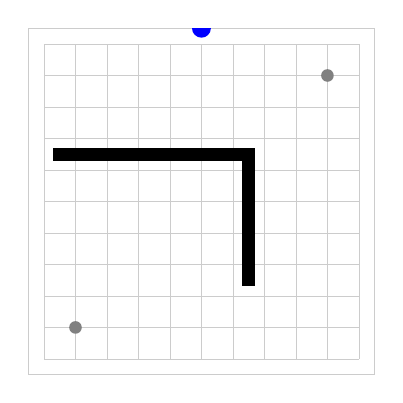
\begin{tikzpicture}[scale=0.4]

\draw[black!20] (-0.5,-0.5) rectangle (10.5,10.5);

\draw[step=1cm,black!20,very thin] (0,0) grid (10,10);

% radars
\begin{scope}
   \clip (-0.5,-0.5) rectangle (10.5,10.5);
   \fill[blue] (5,10.5) circle (0.3cm);

\end{scope}

% obstacles
\fill[black] (0.3,6.3) rectangle (6.7,6.7);
\fill[black] (6.3,2.3) rectangle (6.7,6.3);

\fill[gray] (1.0,1.0) circle (0.2cm);
\fill[gray] (9.0,9.0) circle (0.2cm);
\end{tikzpicture}
\end{document}
